\subsection{Order of Accuracy of C1FR}
\subsubsection{Setup}

The 1-D experiments follow the procedure suggested by Vincent et al.~\cite{vincent2011insights} to estimate  a scheme's order of accuracy isolating interpolation errors. We solve the linear advection equation with advection speed of $a = 1$. The domain was $\Omega = [-10, 10]$ and was discretized in $n = 10, 15, 24, 38, 60$ equispaced elements of orders $P = 1,2,3$. The initial condition was a sine wave with wavenumber $k = 2\pi/20 \approx 0.63$. The advection speed was $1$ and fully upwinded fluxes $\alpha_0 = 0, \alpha_1 = 0$ in Eqn. \eqref{eq:ifluxdef}) were used. The boundary conditions were periodic. The simulation advanced using a fourth order \gls{rk} scheme with a time-step of order $10^{-3}$.

The initial condition was advected for a full domain length, using either standard nodal DG or \gls{c1fr}, and the resulting solution was taken as the reference solution $u_{ref}$. The wave was advected for a further full domain length to obtain the final solution $u_{final}$. The error was calculated by taking the L-2 norm of $u_{ref} - u_{final}$.

\subsubsection{Results and discussion}
Figures \ref{fig:adv_P1},\ref{fig:adv_P2}, and \ref{fig:adv_P3} show the rate of convergence of the solution and its derivative obtained by discretizing the solution wih polynomials of order $P = 1,2,3$, respectively. The slopes of the best fit lines are presented in each figure's caption.

\begin{figure}[h]
\centering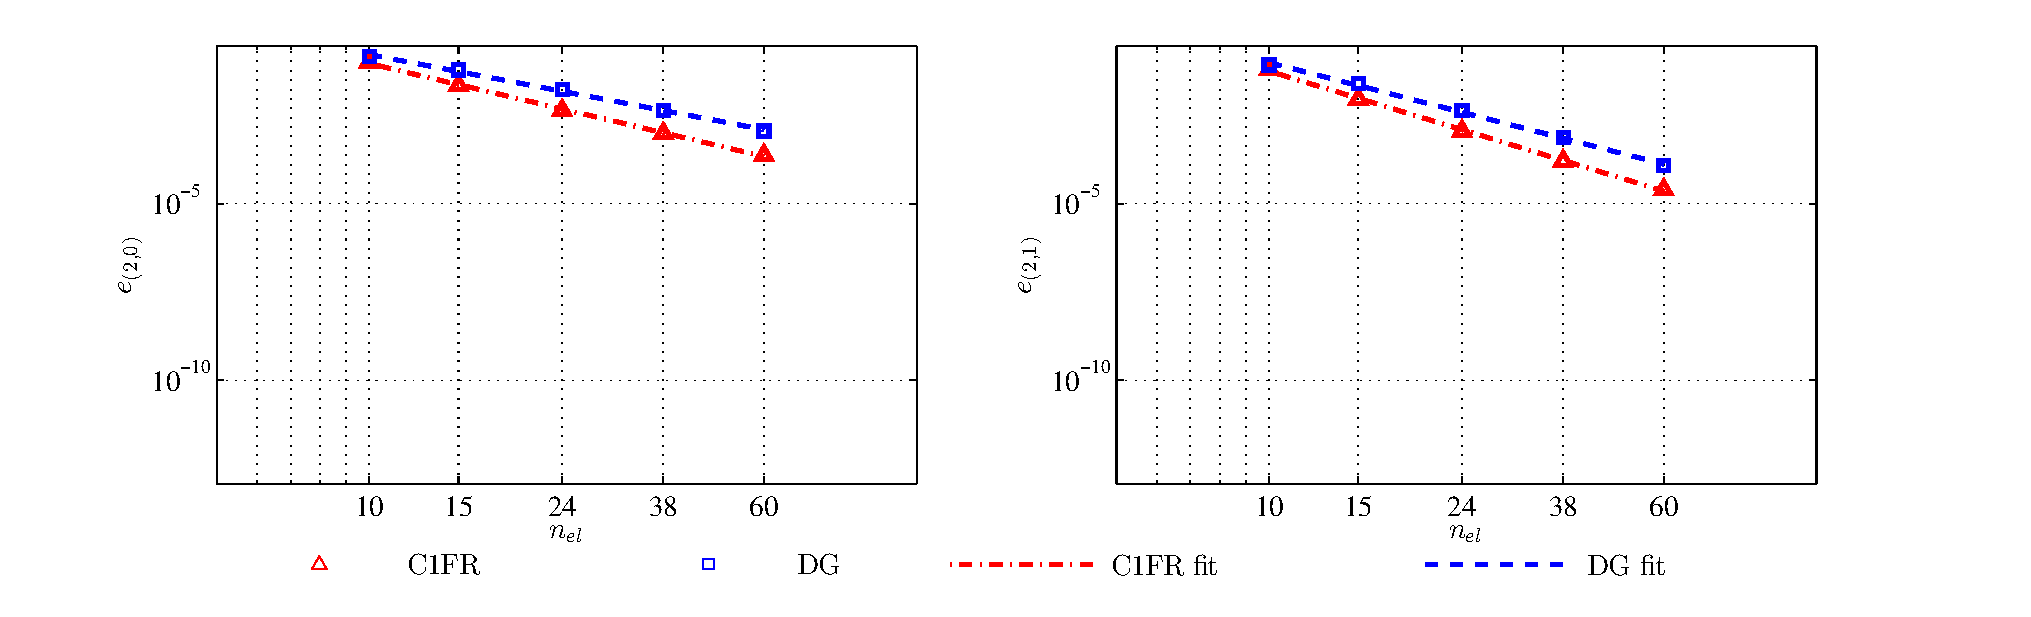
\includegraphics[width=1\textwidth,trim=\Ltrim cm 0cm \Rtrim cm 0cm]{\cmfrdir/Figures/Order_accuracy/P_1}
\caption{L-2 norm of error of advected sine wave and its derivative, $e_{(2,0)}$ and $e_{(2,1)}$ respectively, versus number of elements, for linear advection with polynomial discretization of order $P = 1$. Order of accuracy in solution: \gls{dg}: $2.728$, \gls{c1fr}: $3.374$. Order of accuracy in first derivative: \gls{dg}: $2.691$, \gls{c1fr}: $3.359$.}
\label{fig:adv_P1}
\end{figure}

\begin{figure}[h]
\centering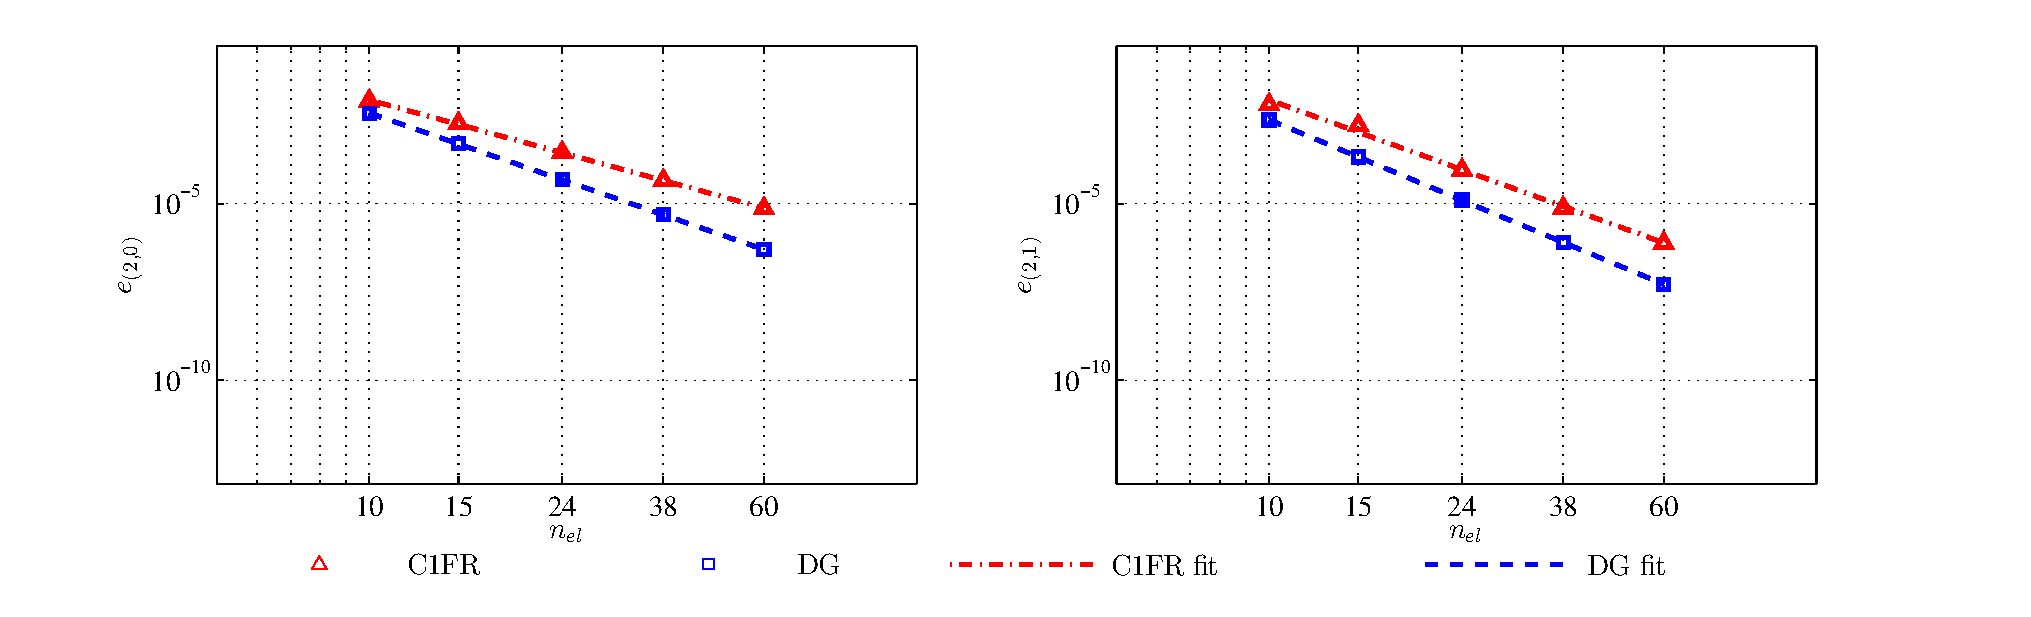
\includegraphics[width=1\textwidth,trim=\Ltrim cm 0cm \Rtrim cm 0cm]{\cmfrdir/Figures/Order_accuracy/P_2}
\caption{L-2 norm of error of advected sine wave and its derivative, $e_{(2,0)}$ and $e_{(2,1)}$ respectively, versus number of elements, for linear advection with polynomial discretization of order $P = 2$. Order of accuracy in solution: \gls{dg}: $4.960$, \gls{c1fr}:  $3.917$ . Order of accuracy in first derivative: \gls{dg}: $4.971$, \gls{c1fr}: $4.178$.}
\label{fig:adv_P2}
\end{figure}

\begin{figure}[h]
\centering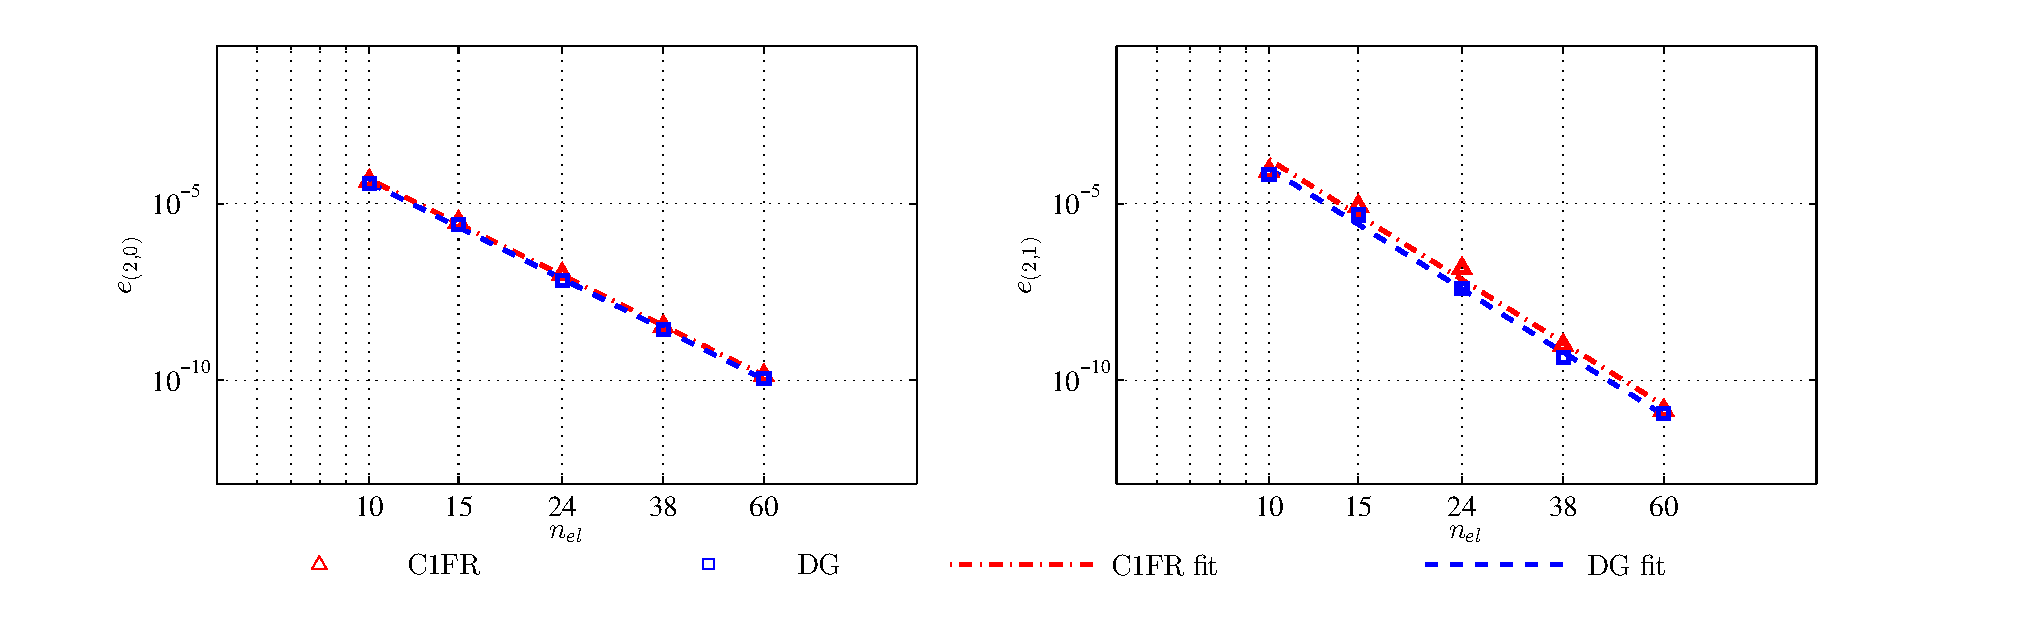
\includegraphics[width=1\textwidth,trim=\Ltrim cm 0cm \Rtrim cm 0cm]{\cmfrdir/Figures/Order_accuracy/P_3}
\caption{L-2 norm of error of advected sine wave and its derivative, $e_{(2,0)}$ and $e_{(2,1)}$ respectively, versus number of elements, for linear advection with polynomial discretization of order $P = 3$. Order of accuracy in solution: \gls{dg}: 7.119, \gls{c1fr}: 7.187. Order of accuracy in first derivative: \gls{dg}: 7.908, \gls{c1fr}: 7.882.}
\label{fig:adv_P3}
\end{figure}

The fact that we recover the expected nodal \gls{dg}'s $2P+1$ order of convergence found by Vincent et al. \cite{vincent2011insights} for $P = 1,2,3$ validates the experimental setup. It is interesting to note that \gls{c1fr} retains \gls{fr}'s even-odd order of convergence behavior: when $P$ is odd, the order of convergence is $2P+1$; while when $P$ is even, the order of convergence is $2P$.

This numerical experiment does not replace a von Neumann analysis, but does show that the scheme is stable, consistent, and maintains the desired order of accuracy. Although we would not expect the scheme to maintain super-convergence properties in real applications --as the interpolation errors are themselves of order $P+1$--, this experiment relieves worries about C1FR's introducing lower order errors.